\chapter{Application Programming Interfaces}


Some Application Programming Interfaces (APIs) have been written that mimics more or less the inline commands behavior: instead of specifying a number of control parameters (that may change because of code evolution), the user only have to give a pointer to a string (\texttt{char *}) containing the control parameters that he/she would have given in a inline command. 

API procedure are named after the inline command, i.e. for the inline command \blockmatching, the API procedure is named \texttt{API\_blockmatching}.

\begin{attention}
Typically, the inline command has only to deal with the I/O (reading the input structures, e.g. images or transformation, and writing the result structures after processing), while the processing takes place in the API procedure.

However, because of already existing interfaces, and to keep a backward compatibility, a more complex scheme may have to be built, see e.g. the \blockmatching API in section \ref{sec:api:blockmatching}.
\end{attention}


\section{\blockmatching API}
\label{sec:api:blockmatching}

\begin{figure}[ht]
\begin{center}
 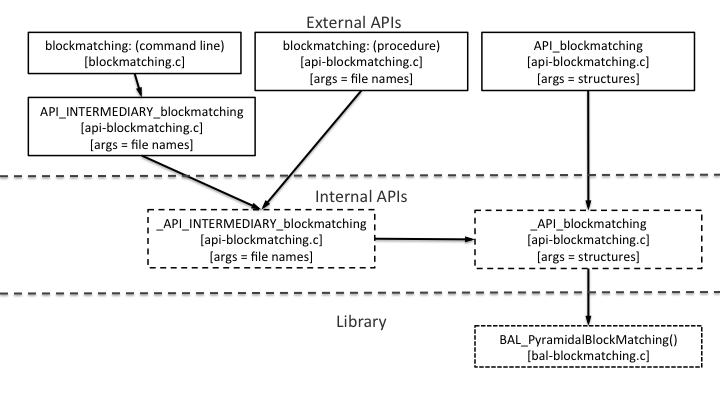
\includegraphics[width=0.8\linewidth]{figures/api-blockmatching.png}
\end{center}
\caption{\label{fig:api:blockmatching} Organization of the blockmatching related APIs.}
\end{figure}
